% !TEX root = ../new_paper.tex
We begin with a short set of assumptions: that the DM particle, $\chi$, is a weakly interacting Dirac fermion, that it is a singlet under the SM, and that it is the lightest stable new particle. We also require minimal flavour violation (MVF) to hold wherever relevant.
\iffalse
(\comm{Not sure if this is relevant anymore, if we've ditched the scalar model. - Mia})
\fi
Additionally $\chi$ is assumed to couple only to the SM quarks; while coupling to SM leptons \cite{} or gluons \cite{} has been studied elsewhere, it is beyond the scope of this paper. We adopt separate labels for the $s$- and $t$-channel mediators which arise from the resolution of the $q\bar q \rightarrow \chi \chi$ contact interaction of an EFT at tree-level. That is, we denote the $s$-channel mediator, which is taken to be a SM singlet, by $\xi$ and the $t$-channel mediator, which is necessarily charged and coloured, by $\phi$.

The $s$-channel models chosen for analysis are characterised by vector (sV) or axial-vector (sA) couplings to both the dark and SM sectors. 
%In the notation of Ref.~\cite{DMCons2}, these correspond to the D5 and D8 operators respectively in the EFT regime. 
These models are described by the following interaction Lagrangians:
\begin{equation}
\label{L_int_sV}
\mathcal{L}_{sV} = - \xi_{\mu}\left[ \sum\limits_{q} \gq\bar{q}\gamma^{\mu}q - \gX\bar{\chi}\gamma^{\mu}\chi\right],
\end{equation}
\begin{equation}
\label{L_int_sA}
\mathcal{L}_{sA} =  \xi_{\mu}\left[\sum\limits_{q} \gq\bar{q}\gamma^{\mu}\gamma_{5}q - \gX\bar{\chi}\gamma^{\mu}\gamma_{5}\chi\right],
\end{equation}
%\begin{equation}
%\label{L_int_sS}
%\mathcal{L}_{sS} = \sum\limits_{i=1}^{6} g_{q_i}\bar{q_i}q_i\eta + \gX\bar{\chi}\chi\eta,
%\end{equation}
where the sum is over all quarks.
\iffalse
\st{where the sum is over all quarks, $\xi$ is the (axial-)vector mediator and $\chi$ is the dark matter particle - a weakly interacting SM singlet Dirac fermion with mass $\mX$.}
\fi
%\question{The scalar model should really have a Yukawa coupling (ie $\gq \rightarrow \gq m_q / v$) if we want to be consistent with D1 and the ATLAS/CMS run2 simplified models. Is it too late to implement this? - Tom.} \comm{I agree, and this should be easy enough to implement I think. - Amelia}
%\st{For simplicity, it is assumed that both $\xi$ and $\eta$ are SM singlet particles and couple only to pair-antipair combinations of $\chi$ and the SM quarks, with coupling strengths $\gX$ and $\gq$ respectively.}
For the couplings $\gq$ and $\gX$ to remain within the perturbative regime, they are required to satisy $\gq,\gX \leq 4\pi$, though stronger perturbativity requirements do exist \cite{ValidEFT}.
%\bigskip

%\st{Finally, for convenience, the mediator is assumed to couple to }$\cancel{\chi}$\st{ with the same strength as to each of the six quarks, that is, }$\cancel{\gq = \gX \equiv f}$. \comm{Removed, since we want to include cases where this isn't true! - Amelia}
%Note that the vector and axial-vector models have already been studied extensively \cite{Buchmueller:2014yoa, Chatrchyan:2013qha, Aad:2012hf, Harris:2014hga} and so serve as a good basis for the comparison of constraints. \comm{I need to add some citations for the scalar model here - Tom}

The $t$-channel model considered in this paper (abbreviated tS) is characterised by a scalar mediator and is motivated by analogy with a common aspect of Supersymmetric models: neutralino DM interacting with the SM sector via $t$-channel exchange of a squark \cite{SUSYDM}. Note that in this Supersymmetric scenario the DM particle is a Majorana fermion. SiMs in which $\chi$ is of Majorana type are kinematically identical to the corresponding Dirac cases (requiring multiplication of the cross-section by a simple factor in order to compute limits) and so are not covered here (the exception being in the validation of the \monoZ channel, see Sec. \ref{monoZ_validation}). The exception to this rule is the $s$-channel vector mediator model, which vanishes if $\chi$ is a Majorana fermion \cite{METSig}.
%\bigskip

In the tS model, the mediator is allowed to couple to either the left or right-handed quarks as a SU(2) doublet or singlet respectively. Since the LHC is insensitive to the chirality of the quarks, we assume for simplicity that $\phi$ couples to the left-handed quarks only. We also assume that the masses and couplings of $\phi$ are equal across the three generations, and that the masses of the two components of $\phi$ are equal. The interaction Lagrangian for this model is then:
\begin{equation}
\label{L_int_tS}
\mathcal{L}_{tS} = \sum_{Q} \gqX \bar{Q} P_R \phi \chi + {\rm h.c.},
\end{equation}
where the sum is over the three $Q_L$ doublets, $\gqX$ is the scalar coupling of the incoming quark, $\phi$ and $\chi$, and $P_R$ is the usual chiral projection operator.

% THOMAS!! Do we need to rewrite the Lagrangian for TSD? ie is this consistent with our UFO?

\iffalse
\hspace{1cm}\textcolor{blue}{\st{When constraining the above models using the collider production cross-section for the process }$\cancel{pp \rightarrow X + \bar{\chi}\chi}$\st{ it is also important to consider the impact of the mediator decay width, }$\cancel{\Gamma}$ \cite{}\st{. The reason being that }$\cancel{\sigma\left(pp \rightarrow X + \bar{\chi}\chi\right)}$\st{ scales as:}}
\begin{equation}
\label{cross_section}
\cancel{\frac{f^{4}E^{2}}{(q^{2} - M^{2})^{2} + M^2 \Gamma^{2}}}
\end{equation}
\st{where }$E$\st{ is the centre-of-mass energy of two colliding partons and }$q$\st{ is the four-momentum transferred by the mediator.} \comm{Careful with formulae from other papers, it's caused me enormous headaches in the past when they were wrong :) The formulae we quoted here from \cite{METSig} didn't even have the consistent dimensions! Somehow they dropped the wrong term when squaring the propagator! - Tom.}

\fi

\subsection{Mass and Coupling Points}  % Moved from section 3
We choose to study a representative set of dark matter and mediator masses, shown in Table \ref{Mass_coup_points}. DM masses of 3, 30 and 300 GeV are only included in the \monoZ channel. All $\mX-\Mmed$ combinations are permitted in the sV and sA models; in the tS model $\Mmed$ should be greater than $\mX$, to ensure stability of the DM particle. The couplings, $\gq$ and $\gqX$, are set to unity while the DM-mediator coupling, $\gX$, is allowed to vary from this by up to a factor of five for the $s$-channel models. In all cases, a point in phase space is disregarded if it leads to a mediator width greater than 50\% of the mediator mass, as will be further discussed below. The mediator masses were chosen to cover a broad range of parameter space and to coincide with predominantly three regimes: (near-)degenerate ($\Mmed \approx \mX$), kinematically allowed ($\Mmed \geq 2 \mX$), and EFT-like ($\sqrt{\hat{s}} << \Mmed $) \footnote{A recent study by Alves et al. found that EFT results do not apply to mediators with a mass less than 2.5 TeV at the LHC during Run I \cite{Alves:2011wf}.}. We also allow for the possibility of a light mediator/heavy WIMP scenario ($\Mmed < \mX$) in the sV and sA models.

\begin{table}
\centering
\begin{tabular}{C{3cm} | C{3cm} | C{1.5cm}  C{1.5cm} | C{3cm}}
\hline
\hline
\multirow{2}{*}{$\mX$ [GeV]} & \multirow{2}{*}{$\Mmed$ [GeV]} & \multicolumn{2}{c|} {$s$-channel} & $t$-channel \T \B \\ %\cline{3-5}
& & $\gq$ & $\gX$ & $\gqX$ \T \B\\
\hline
1, (3), 10, (30), 100, (300), 1000 & 1, 2, 10, 20,  100, 200, 1000, 2000, 20 000 & 1 & 0.2, 0.5, 1, 2, 5 & 1 \T \B  \\
\hline
\hline
\end{tabular}
\caption{Mass and coupling points chosen for the analysis of simplified dark matter models. Values in brackets are only included in the \monoZ channel. The mediator masses are primarily representative of three regimes: (near-)degenerate ($\Mmed \approx \mX$), kinematically allowed ($\Mmed \geq 2 \mX$), and EFT-like ($\sqrt{\hat{s}} << \Mmed$). Coupling values that give a mediator width such that $\Gamma_{\mathrm{med}} > 0.5 \times \Mmed$ are not considered. For the $t$-channel model, $\Mmed > \mX$ is also required.}
\label{Mass_coup_points}
\end{table}

\subsection{Width effects}

An important factor when considering simplified models is to ensure the mediator width is treated appropriately, as it impacts both the cross-section calculation and, in some cases, the kinematic behaviour of the model. In previous analyses (ref) it has been common to consider mediators of a fixed width such as $\Gamma = M/8 \pi$  (the minimal width possible with only a single quark helicity coupling to the mediator with $\gq$ = 1), to take advantage of the enhancement in cross section as the width becomes small and on-shell.

In this work, the mediator widths are expanded to include coupling to all kinematically accessible quarks. We assume minimal flavour violation, which implies a universal coupling to all quark flavours. Following $[$(other minimum width papers)$]$, the minimum on-shell kinetic width for each model is given by:

\begin{equation}
  \begin{split}
    \Gamma_{sV} \, = \, & \frac{\gX^2 M}{12\pi}\left(1 + \frac{2 \mX^{2}}{M^{2}}\right)\left(1 - \frac{4 \mX^{2}}{M^{2}}\right)^{\frac{1}{2}} \Theta(M-2 \mX) \\
                  & + \sum_{\substack{q}}\frac{\gq^2M}{4\pi}\left(1 + \frac{2m_{q}^{2}}{M^{2}}\right)\left(1 - \frac{4m_{q}^{2}}{M^{2}}\right)^{\frac{1}{2}} \Theta(M-2m_q)
  \end{split}
\end{equation}

\begin{equation}
  \begin{split}
    \Gamma_{sA} \, = \, & \frac{\gX^2 M}{12\pi}\left(1 - \frac{4 \mX^{2}}{M^{2}}\right)^{\frac{3}{2}} \Theta(M-2 \mX) \\
                  & + \sum_{\substack{q}}\frac{\gq^2 M}{4\pi}\left(1 - \frac{4m_{q}^{2}}{M^{2}}\right)^{\frac{3}{2}} \Theta(M-2m_q) \\
  \end{split}
\end{equation}

\begin{equation}
  \begin{split}
    \Gamma_{tS} \, = \, & \sum_{\substack{q}} \frac{\gqX^2M}{16\pi}\left(1 - \frac{m_{q}^{2}}{M^{2}} - \frac{\mX^{2}}{M^{2}}\right) \\
                  & \times \sqrt{\left(1 - \frac{m_{q}^{2}}{M^{2}} + \frac{\mX^{2}}{M^{2}}\right)^{2} - 4\frac{\mX^{2}}{M^{2}}} \,\, \Theta(M-m_q- \mX) \\
  \end{split}
\end{equation}

The expressions for width above are valid where that width is smaller than the mass of the mediator. Moreover, a recent paper [Tom+Karl, others?] demonstrated that the MadGraph treatment of the mediator as a Breit-Wigner propagator, rather than a true kinetic propagator, is accurate only up to $\Gamma \lesssim M/2$. This was also shown to be a necessary requirement for the following approximations regarding the relationship between the couplings and the cross section to hold:

\begin{equation}
  \sigma \propto
  \begin{cases}
      \gq^2 \gX^2 / \Gamma & \mathrm{ if } \Mmed \geq 2 \mDM\\
      \gq^2 \gX^2 & \mathrm{ if } \Mmed < 2 \mDM
  \end{cases}
  \label{eq:sigma_propto_couplings_schan}
\end{equation}
in the sV and sA models, and

\begin{equation}
  \sigma \propto \gqX^4
  \label{eq:sigma_propto_couplings_tchan}
\end{equation}
in the tS model. We find that this requirement fails for a subset of the phase space in the sV and sA models\footnote{Note that the $t$-channel widths are consistently narrower than their $s$-channel counterparts,  as there are six independent mediators compared to the single $s$-channel model mediator.}, and therefore do not include such points in this work.
The impact of varying the mediator width is demonstrated in Fig~\ref{MET_SVD_monoZ}. For the sV and tS models, we plot a simplified $\met$ distribution, as a proxy for the full selection in each analysis, for two and three demonstrative mass points and couplings respectively.  The strength of the coupling directly impacts the width of the mediator in each case. In the \monoZ channel\footnote{In this discussion, the \monoWZ channel can be assumed to follow the same logic as for the \monoZ channel.}, the $\met$ distribution is predominantly independent of the mediator width, and this is also true for the sV model in the \monojet channel. However, there is a clear variation in kinematic behaviour in the tS model in the \monojet channel, which can be attributed to additional diagrams with a gluon in the initial state, accessible in the \monojet channel, which allow the mediator to go on-shell. In this scenario, when the resulting quark and DM particle are both small compared to the mediator mass, they share equally its energy leading to a peak in the $\met$ distribution at approximately half the mediator mass.

In the cases where the model behaviour is independent of the width, we can greatly simplify the calculations by assuming the effect of selection cuts in each channel is constant for each masspoint; that is, independent of the couplings. In this case, a simple rearrangement of eqns.~\ref{eq:sigma_propto_couplings_schan} and \ref{eq:sigma_propto_couplings_tchan} allows us to obtain upper limits on the model couplings (see App.~\ref{Appendix_limitsetting} for further details of this calculation).

Studies of the tS model within the \monojet channel, where scaling the coupling can lead to changed kinematic behaviour, have been performed elsewhere [Papucci], and require the use of iterating the couplings during sample generation. This, combined with the challenges of including differing orders of $\alpha_s$ in the \monojet channel, make the generation process highly computationally expensive compared to the \monoZ and \monoWZ channels, and so we do not consider that particular case here.

%In previous analyses it has been customary to consider mediators of fixed width ranging from $\Gamma = M/8\pi$ to $\Gamma = M/3$ \cite{METSig, Fox:2012ee} \footnote{\textcolor{magenta}{Also add a reference for the recent \monojet paper.}}. This approach is motivated by the observation that, where the mediator is exchanged in the $s$-channel and produced on-shell, $\sigma\left(pp \rightarrow X + \bar{\chi}\chi\right)$ is maximally enhanced when $\Gamma$ is small\footnote{For a more in depth discussion see Ref. \cite{METSig}.}. The smallest width, $\Gamma = M/8\pi$, corresponds to a mediator which couples only to one helicity and flavour of quark with $\gq = 1$ \cite{METSig}. In this paper, the mediator widths are expanded to include coupling to all kinematically accessible quark flavours. We also allow for flavour-blind coupling (when not restricted by MFV), so our definition of the minimum width must change to reflect this. Following $[$(other minimum width papers)$]$, the minimum width for each model is given by:

%The expressions for width above are valid where that width is smaller than the mass of the mediator; moreover, a recent paper [Tom+Karl] demonstrated that the MadGraph treatment of the particle width is accurate only up to $\Gamma < \frac{M}{2}$. We find this to hold true in all cases where the couplings are set to unity, and violated in a set of $s$-channel cases where the coupling ratio satisfies $\frac{\gX{\gq} \geq 2$. These points in phase space are therefore not included in this work.

%\begin{equation}
%\label{Xsec_sim_coupling4}
%(\gq \gX)_{\mathrm{lim}} = (\gq \gX)_{\mathrm{gen}} \times \left ( \frac{\sigma_{\mathrm{lim}}}{\sigma_{\mathrm{gen}}} \right )^{\frac{1}{2}}
%\end{equation}
%where uncertainties are ignored for now. This approximation also relies on the kinematic behaviour of the model to remain relatively stable as the coupling varies, where any variation is introduced by the width. To be more explicit about this: the shape of, say, the MET distribution leads fairly directly to an acceptance, which is then converted into a limit on the visible cross section, and then converted to a limit on the coupling, which may be quite different from the coupling value that was used to estimate the MET distribution. If the MET distribution is stable, we could expect similar acceptances for different coupling values, and the process and eq \ref{Xsec_sim_coupling4} are valid. On the other hand, if the MET distribution is heavily dependent on the width/coupling, the limiting value of the coupling as calculated above would produce a quite different MET distribution to that used to calculate the limit, invalidating the equation. The required process then is to create samples with varied couplings and calculate the limit in each case, and repeat until the generated value and the calculated limit converge.

\begin{figure}[t]
  \begin{center}
    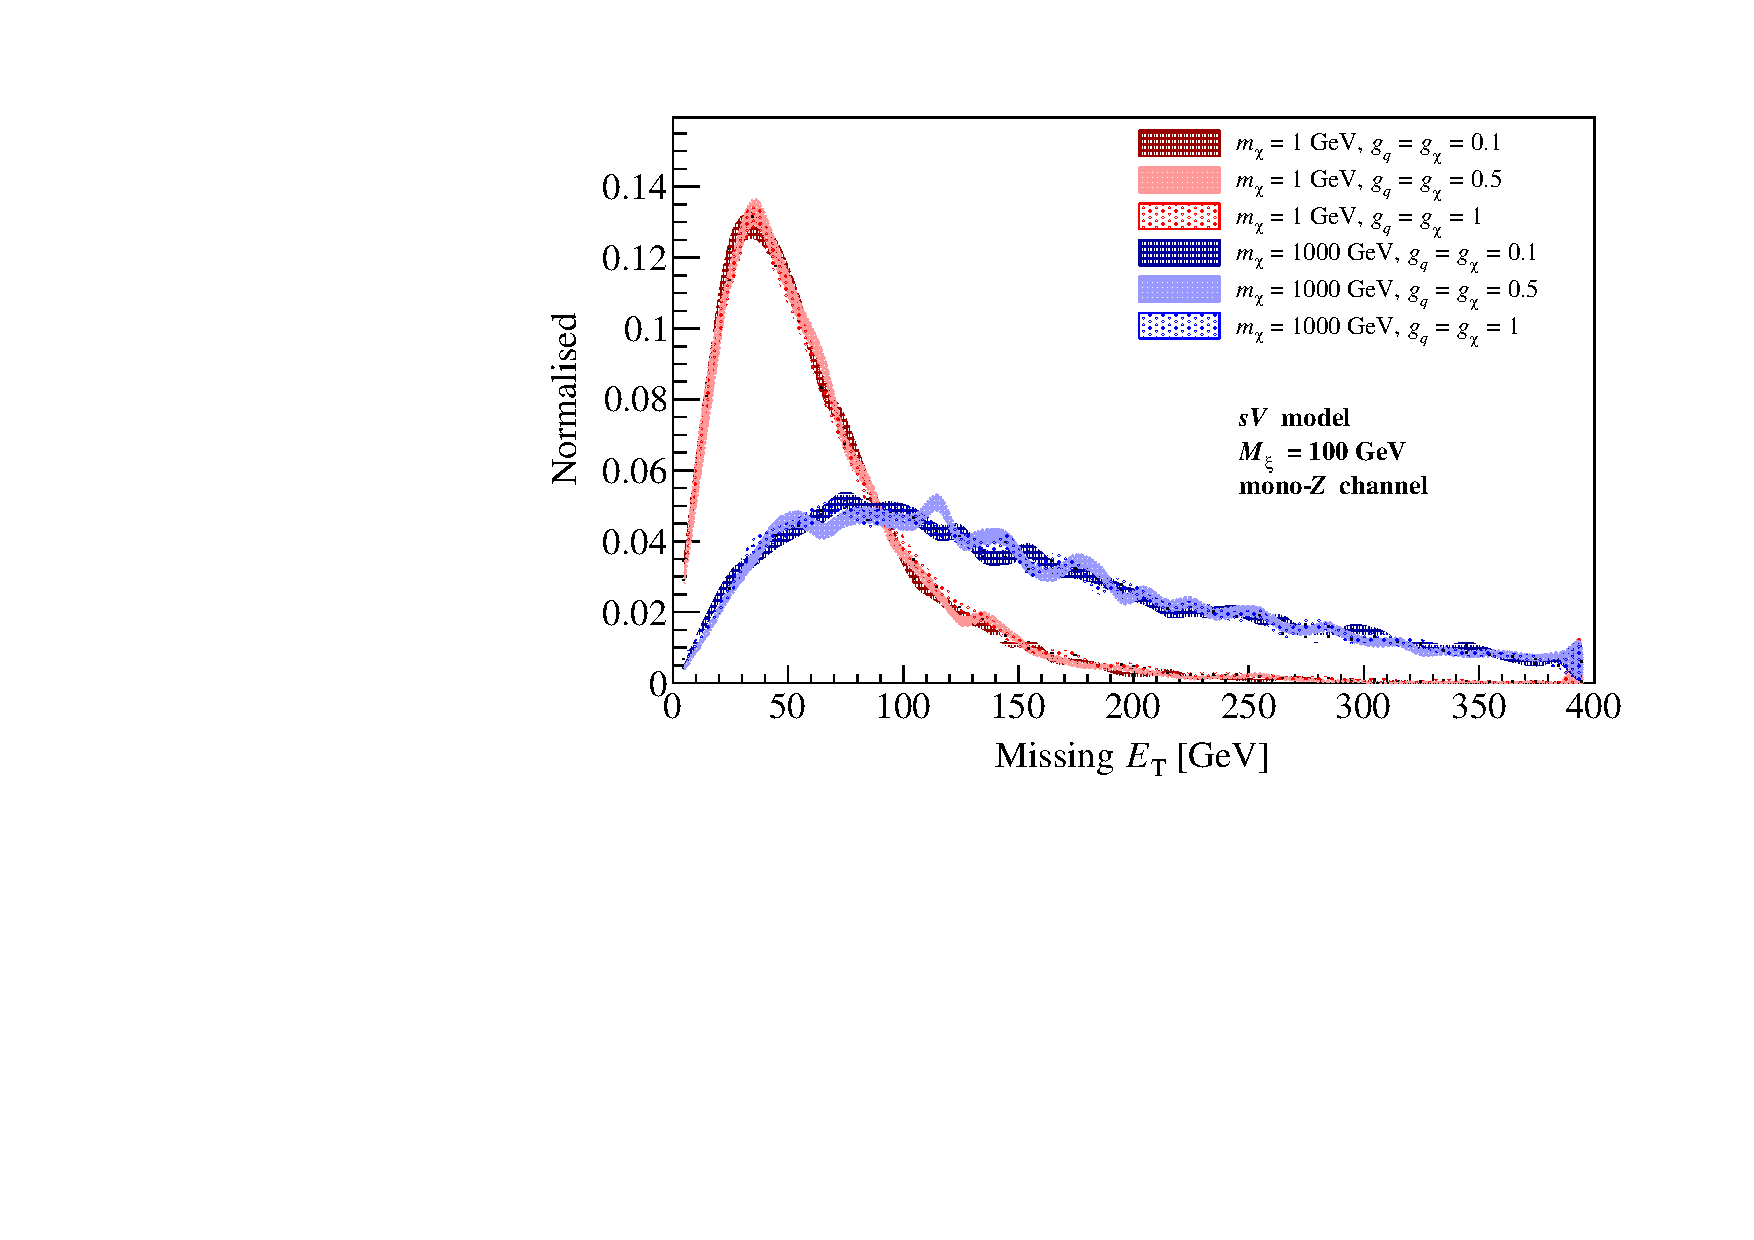
\includegraphics[width=0.45\textwidth]{figures/SVD_MET.pdf}
    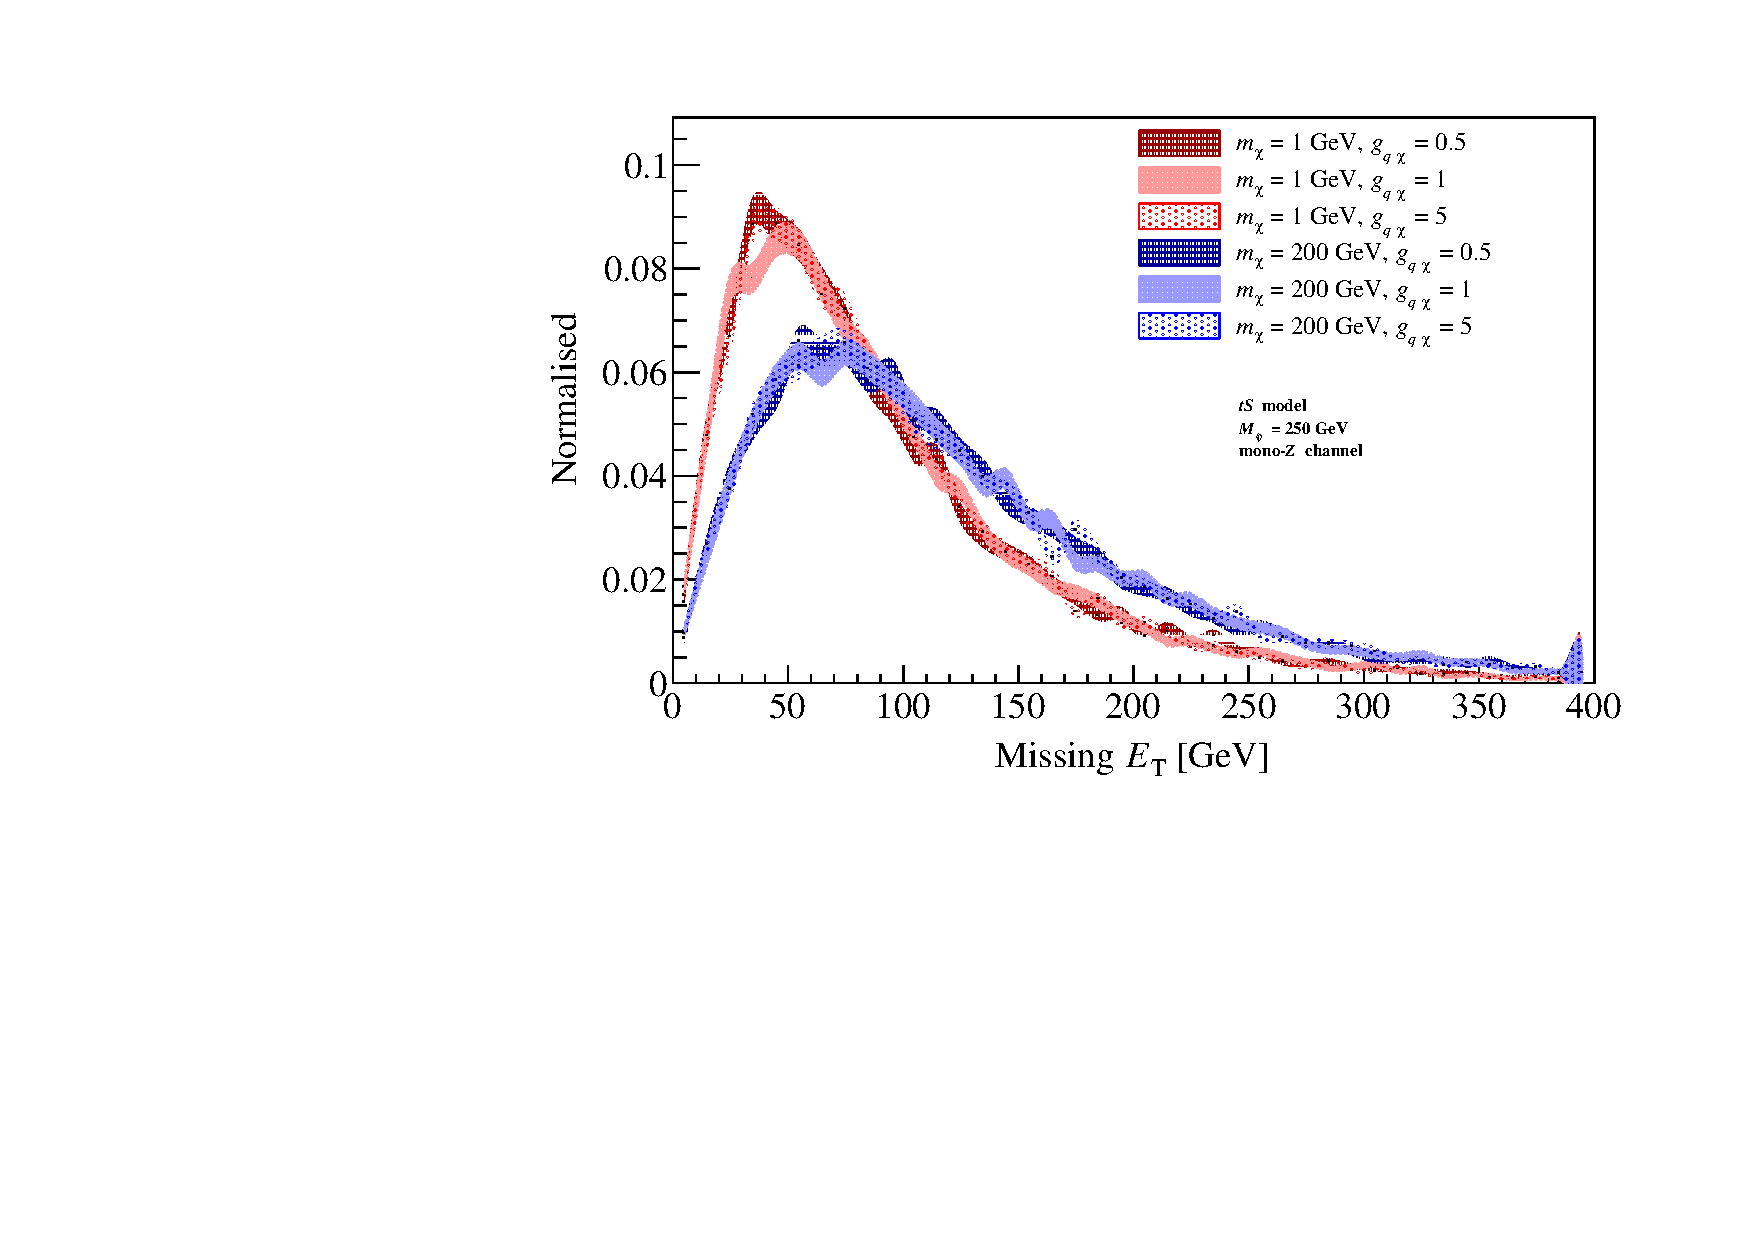
\includegraphics[width=0.45\textwidth]{figures/TSD_MET.pdf}
    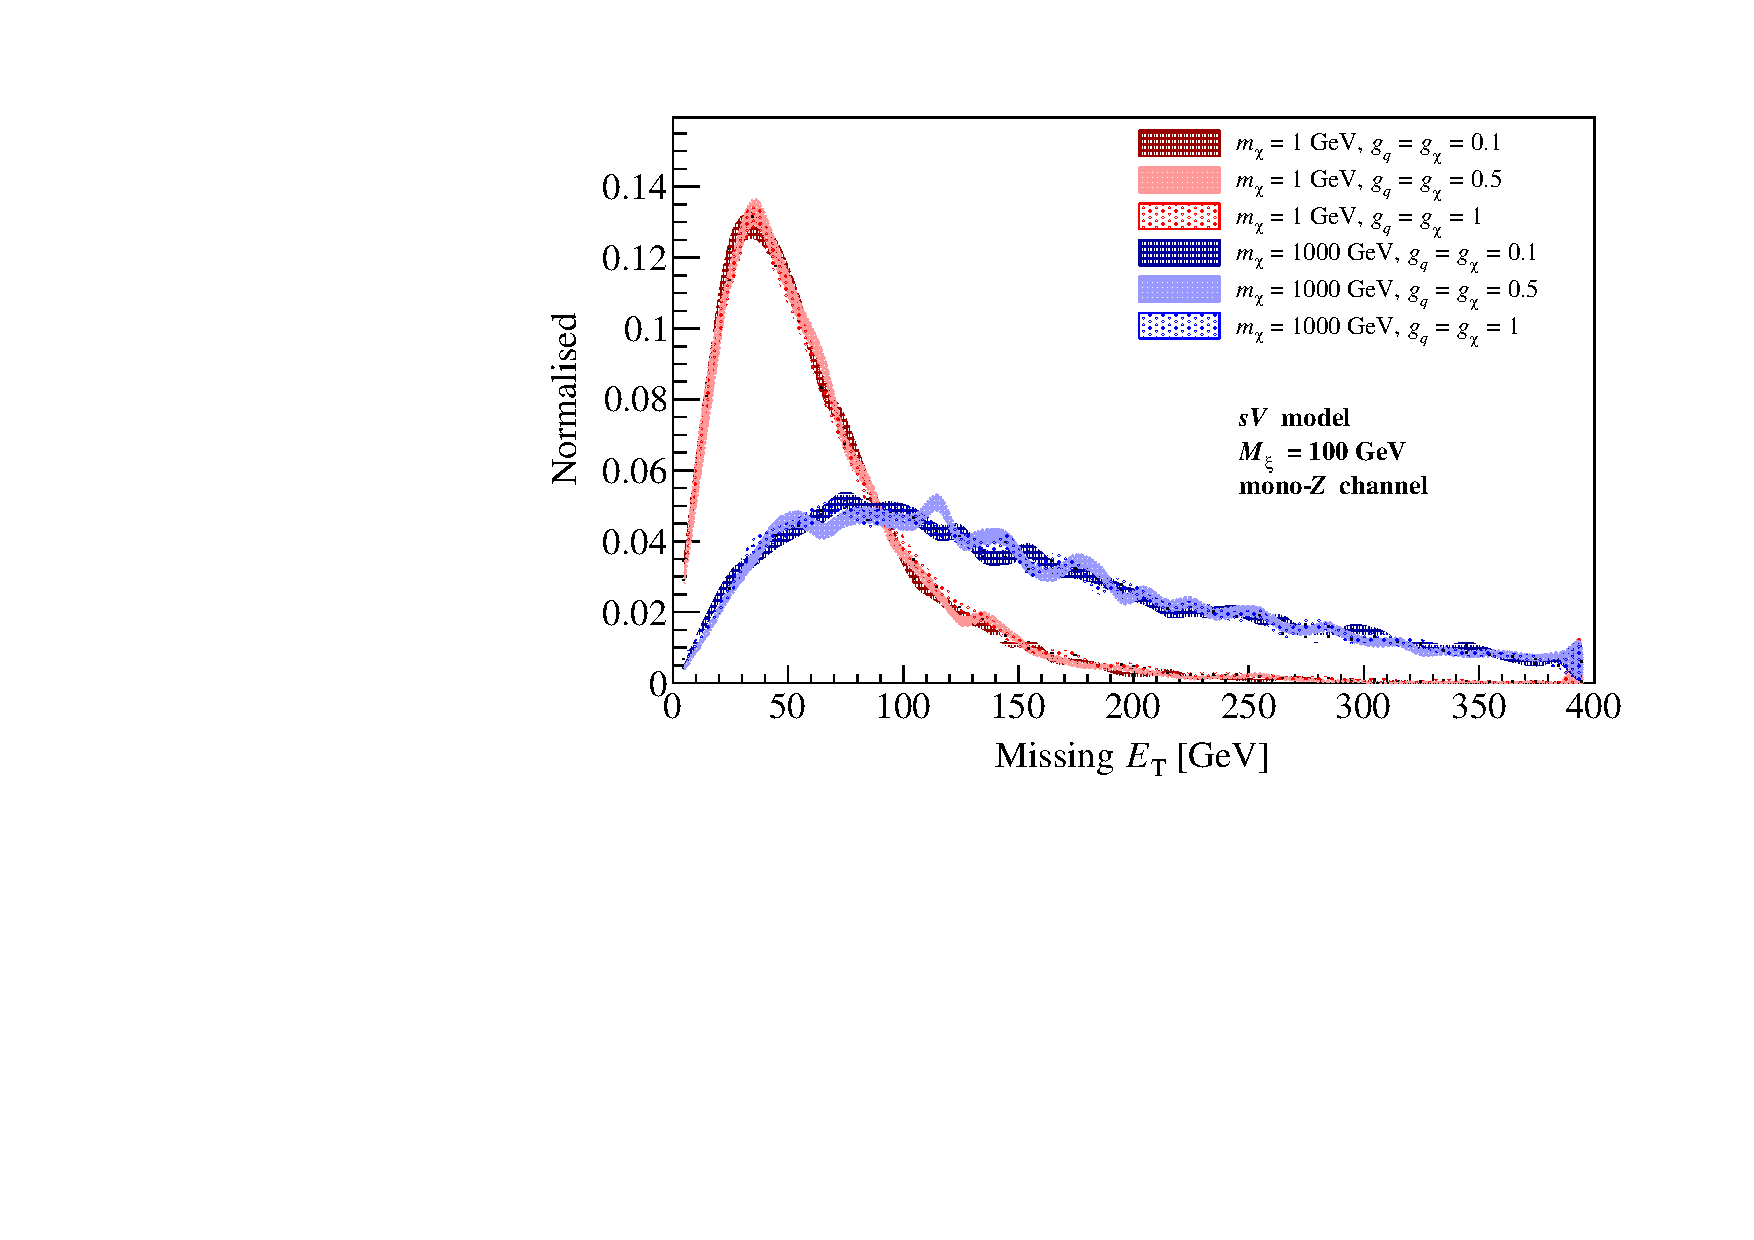
\includegraphics[width=0.45\textwidth]{figures/SVD_MET.pdf}
    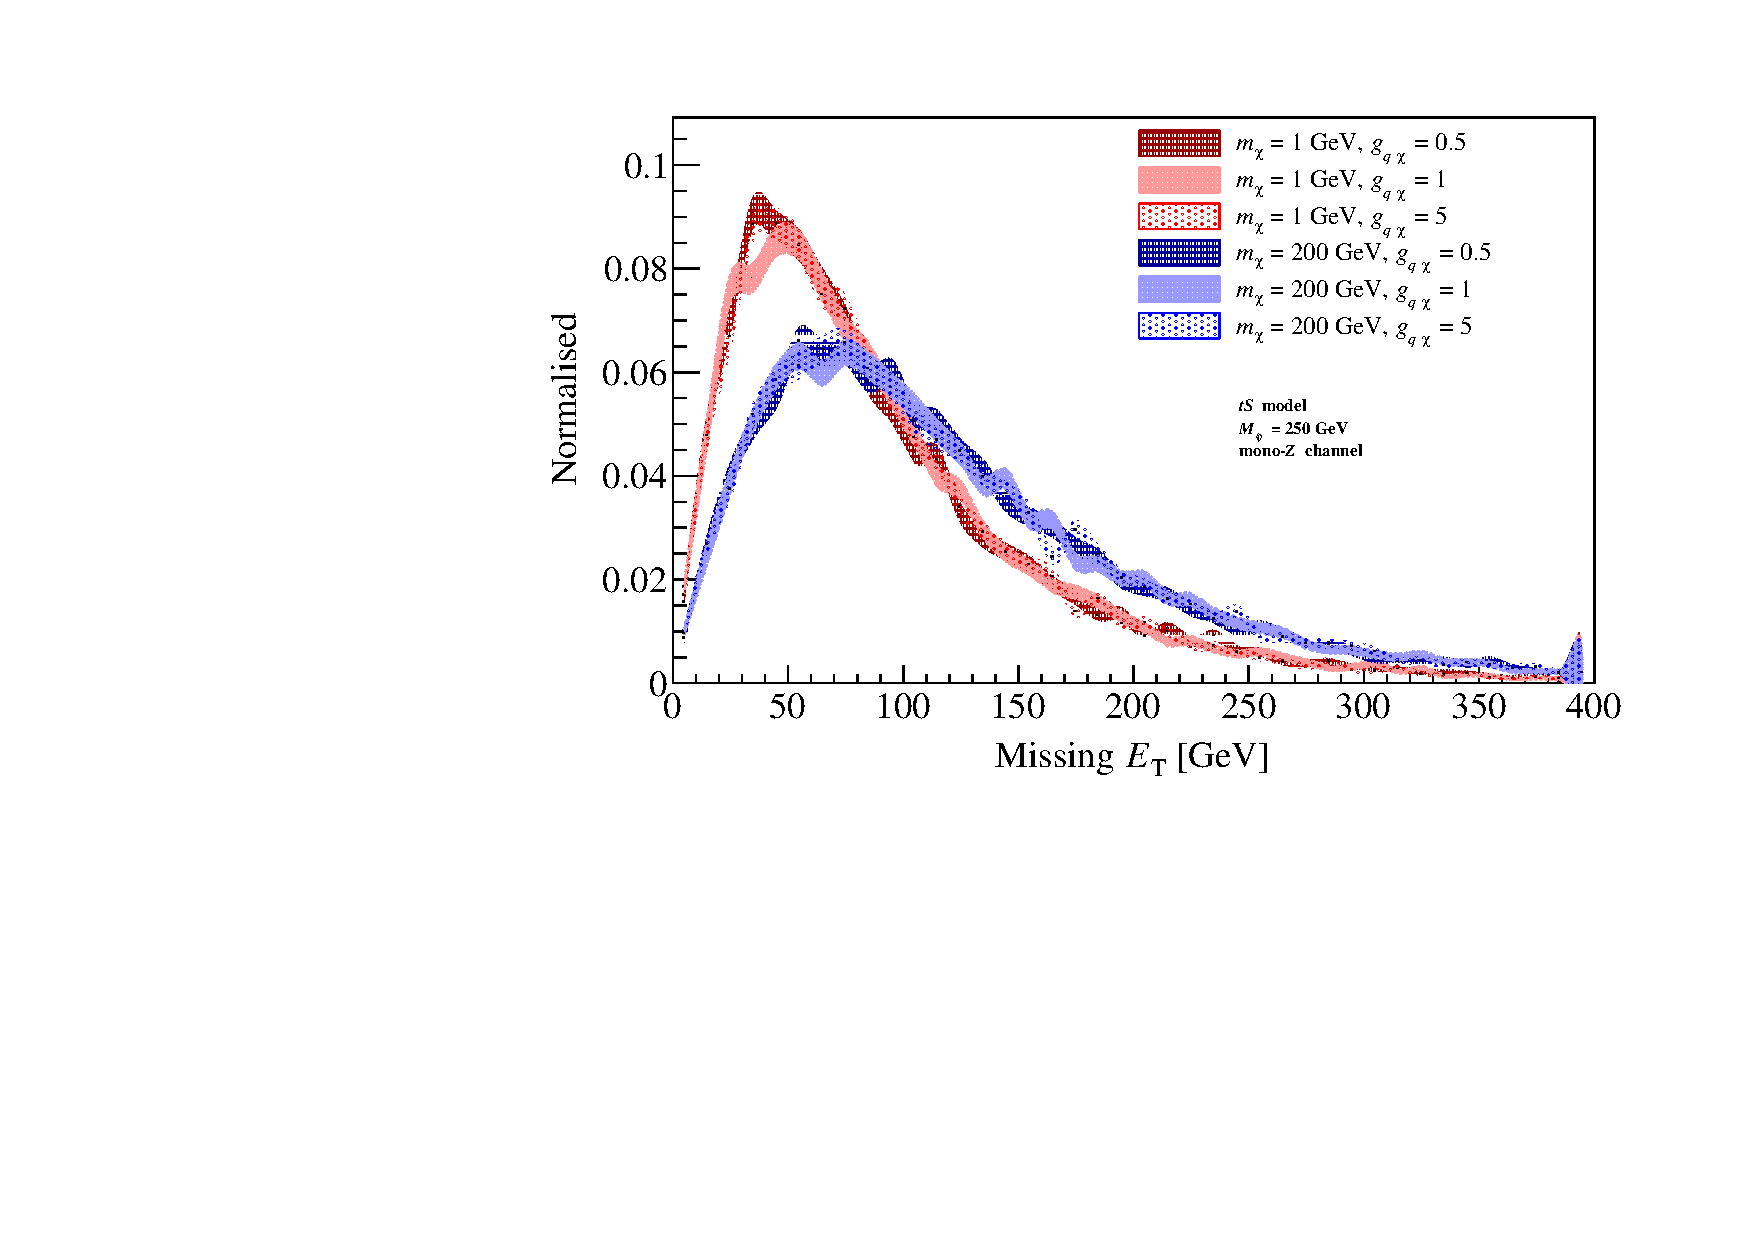
\includegraphics[width=0.45\textwidth]{figures/TSD_MET.pdf}
    \caption{The $\met$ distribution showing the lack of dependence on the coupling (and hence the width) - possibly should include the widths on the plot. Top plots should be replaced with \monojet case.}
    \label{MET_SVD_monoZ}
  \end{center}
\end{figure}

%\textcolor{magenta}{This section should include:}
%\begin{enumerate}
%\item \textcolor{magenta}{Brief motivation for choice of simplified models? (eg. something like "we consider the most straightforward UV-completions of the D1, D5 and D8 effective operators, corresponding to the s-channel scalar, vector and axial-vector models respectively.}
%\item \textcolor{magenta}{The interaction Lagrangians for our four SiMs along with an explanation for why we only assume coupling to SM quarks.}
%\item \textcolor{magenta}{The assumptions and the decay widths associated with our models (?).}
%\item \textcolor{magenta}{Comments on the requirement that $\sqrtgqgX} \leq 4\pi$ in order for the theory to remain perturbative? $\rightarrow$ comments on the choice of mass and coupling points used? Or does this belong in section \ref{sec:sec3}?}
%\end{enumerate}

%Resolving the mediator leads to two possibilities: the mediating particle is exchanged in the s-channel, in which case it may be colour neutral, or it is exchanged in the t-channel in which case it is necessarily coloured \cite{}.

%\cite{ValidEFT, BeyondEFT, CSUSY} t-channel \cite{Buchmueller:2014yoa, SiM}.
